%-------------------------
% Resume in Latex
% Author : Jake
% % License : MIT
%------------------------

\documentclass[letterpaper,11pt]{article}

\usepackage{latexsym}
\usepackage{fullpage}
\usepackage{titlesec}
\usepackage{marvosym}
\usepackage[usenames,dvipsnames]{color}
\usepackage{verbatim}
\usepackage{enumitem}
\usepackage[hidelinks]{hyperref}
\usepackage{fancyhdr}
\usepackage[english]{babel}
\usepackage{tabularx}
\usepackage{graphicx}
\input{glyphtounicode}


%----------FONT OPTIONS----------
% sans-serif
% \usepackage[sfdefault]{FiraSans}
% \usepackage[sfdefault]{roboto}
% \usepackage[sfdefault]{noto-sans}
% \usepackage[default]{sourcesanspro}

% serif
% \usepackage{CormorantGaramond}
% \usepackage{charter}


\pagestyle{fancy}
\fancyhf{} % clear all header and footer fields
\fancyfoot[R]{\thepage\ of 2}
\renewcommand{\headrulewidth}{0pt}
\renewcommand{\footrulewidth}{0pt}

% Adjust margins
\addtolength{\oddsidemargin}{-0.5in}
\addtolength{\evensidemargin}{-0.5in}
\addtolength{\textwidth}{1in}
\addtolength{\topmargin}{-.5in}
\addtolength{\textheight}{1.0in}

\urlstyle{same}

\raggedbottom
\raggedright
\setlength{\tabcolsep}{0in}

% Sections formatting
\titleformat{\section}{
  \vspace{-4pt}\scshape\raggedright\large
}{}{0em}{}[\color{black}\titlerule \vspace{-5pt}]

% Ensure that generate pdf is machine readable/ATS parsable
\pdfgentounicode=1

%-------------------------
% Custom commands
\newcommand{\resumeItem}[1]{
  \item\small{
    {#1 \vspace{-2pt}}
  }
}

\newcommand{\resumeSubheading}[4]{
  \vspace{-2pt}\item
    \begin{tabular*}{0.97\textwidth}[t]{l@{\extracolsep{\fill}}r}
      \textbf{#1} & #2 \\
      \textit{\small#3} & \textit{\small #4} \\
    \end{tabular*}\vspace{-7pt}
}

\newcommand{\resumeSubSubheading}[2]{
    \item
    \begin{tabular*}{0.97\textwidth}{l@{\extracolsep{\fill}}r}
      \textit{\small#1} & \textit{\small #2} \\
    \end{tabular*}\vspace{-7pt}
}

\newcommand{\resumeProjectHeading}[2]{
    \item
    \begin{tabular*}{0.97\textwidth}{l@{\extracolsep{\fill}}r}
      \small#1 & #2 \\
    \end{tabular*}\vspace{-7pt}
}

\newcommand{\resumeSubItem}[1]{\resumeItem{#1}\vspace{-4pt}}

\renewcommand\labelitemii{$\vcenter{\hbox{\tiny$\bullet$}}$}

\newcommand{\resumeSubHeadingListStart}{\begin{itemize}[leftmargin=0.15in, label={}]}
\newcommand{\resumeSubHeadingListEnd}{\end{itemize}}
\newcommand{\resumeItemListStart}{\begin{itemize}}
\newcommand{\resumeItemListEnd}{\end{itemize}\vspace{-5pt}}

%-------------------------------------------
%%%%%%  RESUME STARTS HERE  %%%%%%%%%%%%%%%%%%%%%%%%%%%%


\begin{document}

%----------HEADING----------
\noindent
\begin{tabular*}{\textwidth}{m{5cm}@{\hspace{0.5cm}}m{0.65\textwidth}}
  \centering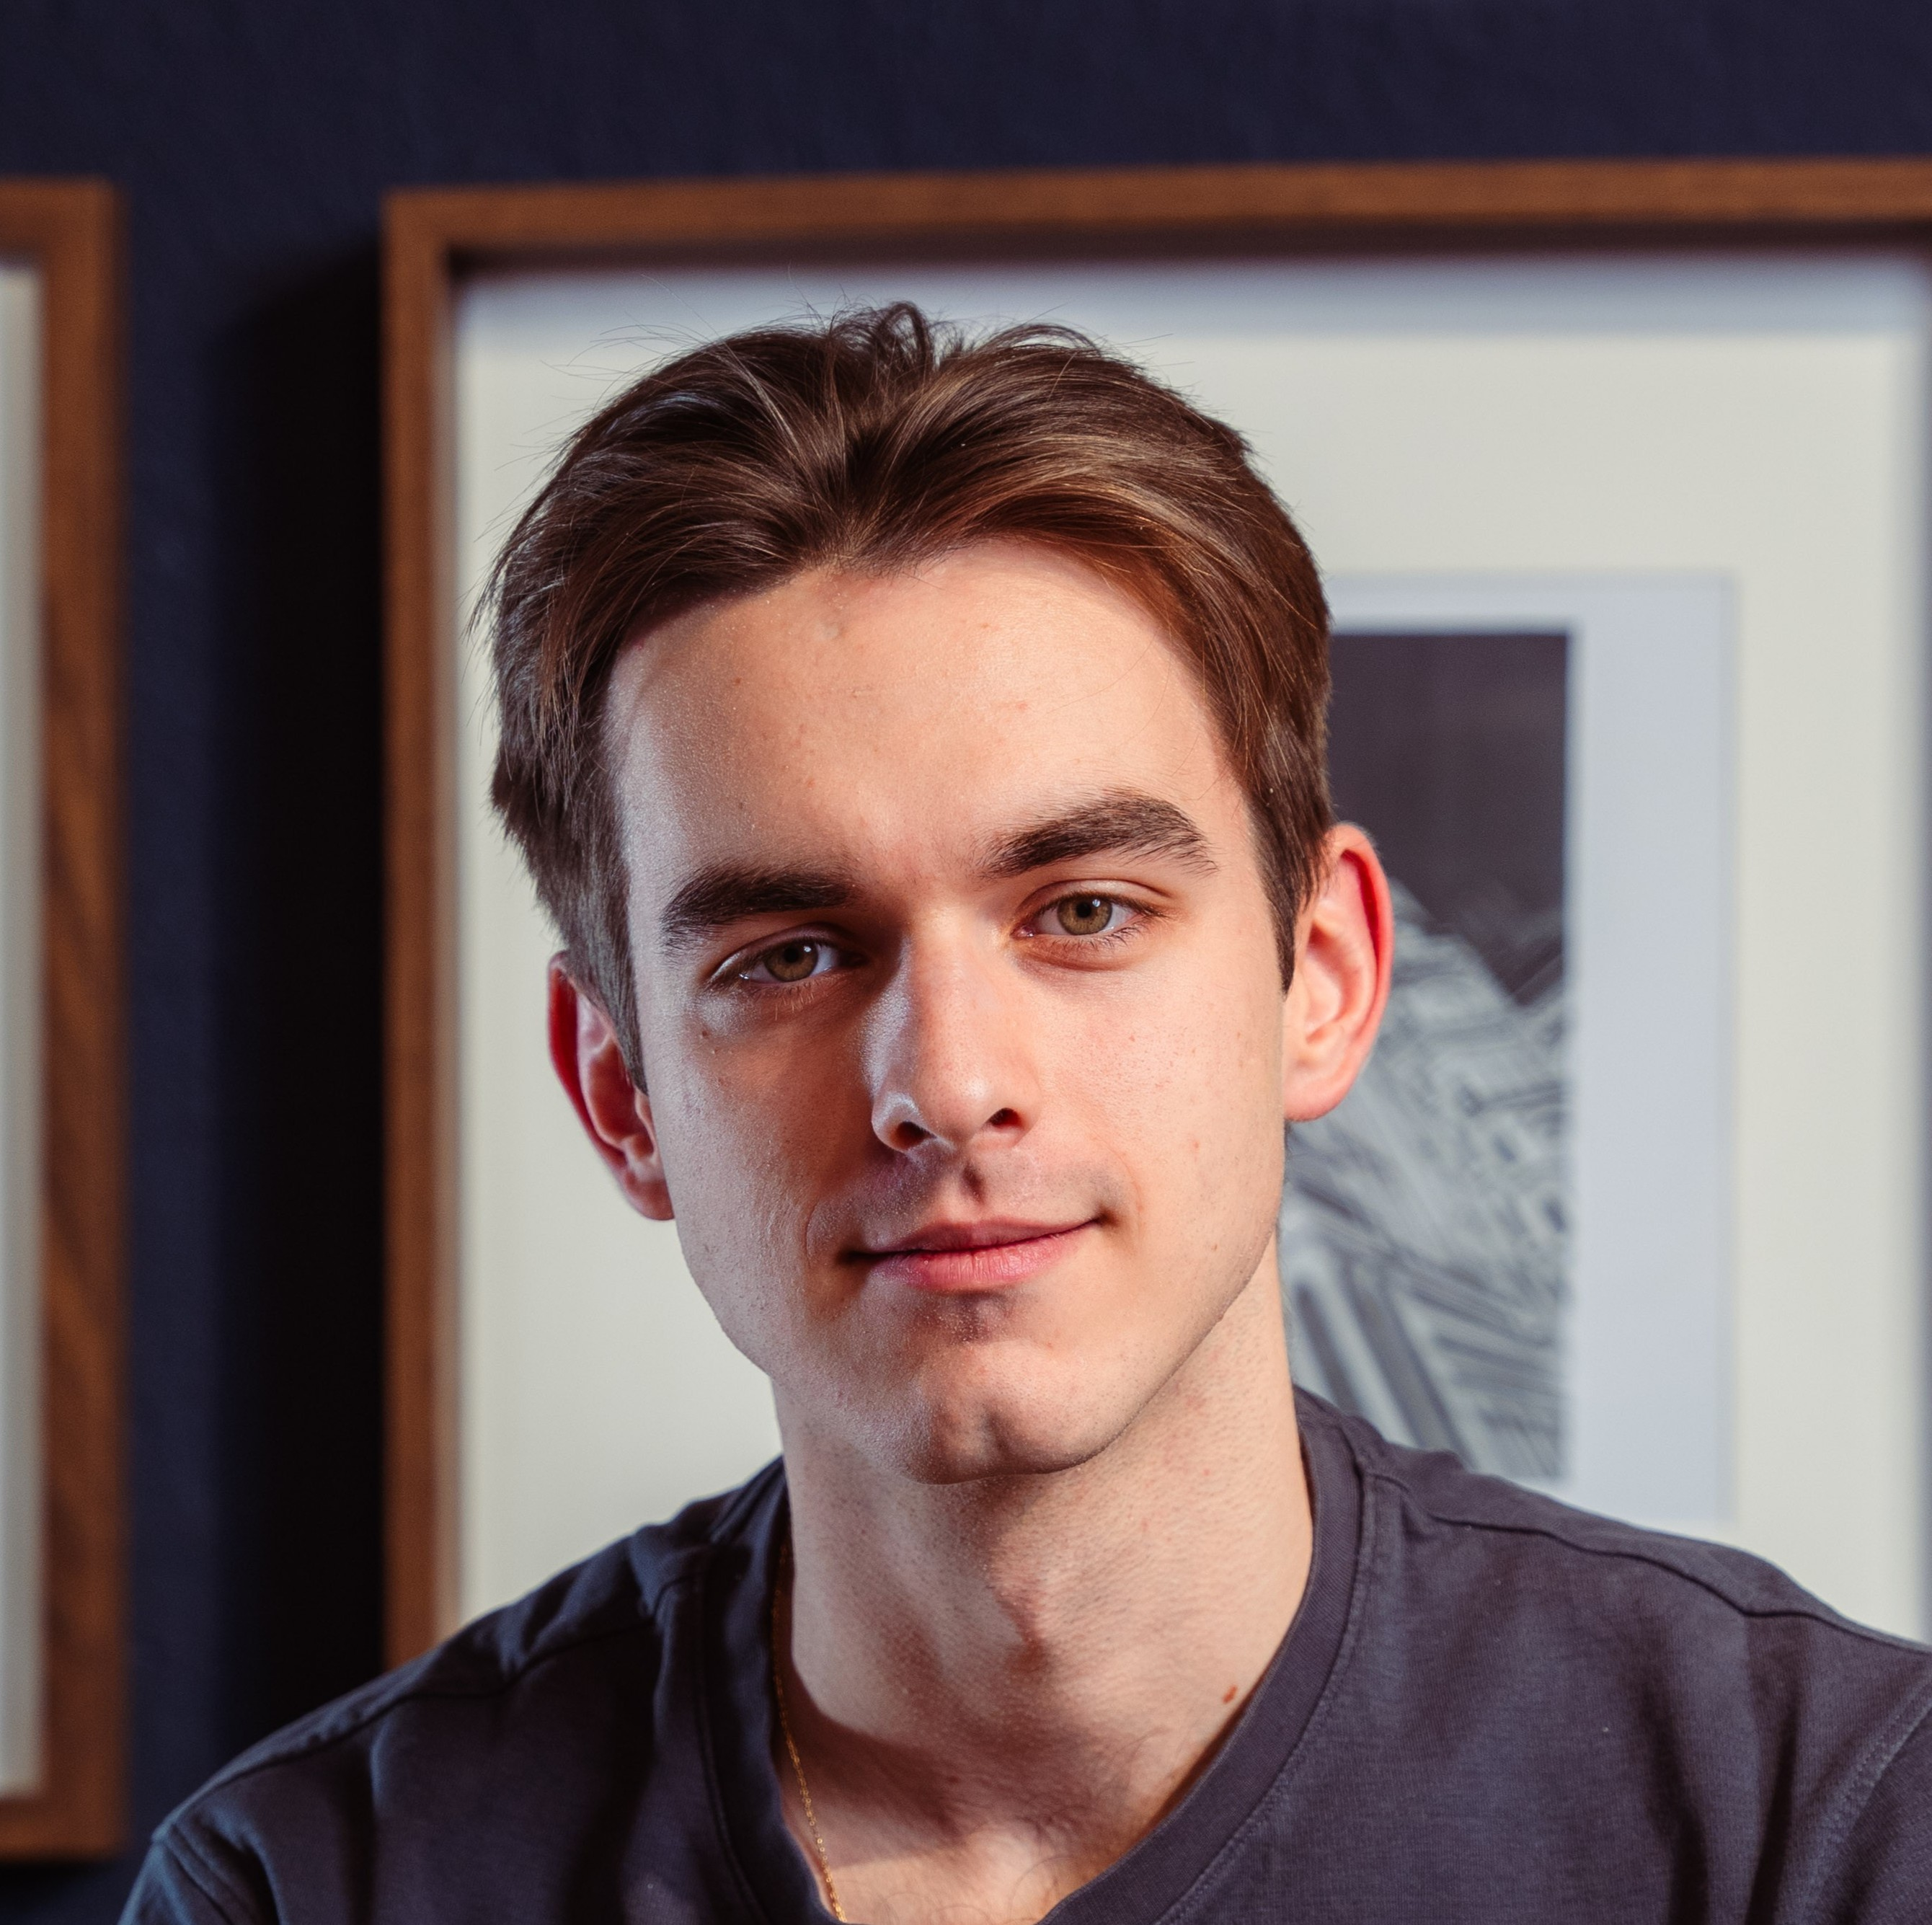
\includegraphics[height=5cm,keepaspectratio]{me.jpg} &
  \begin{minipage}[c]{0.65\textwidth}
    \textbf{\Huge \scshape Petru Popa} \\[6pt]
    \textbf{\small CS BSc University of Bucharest} \\
    \small \href{https://www.linkedin.com/in/petru-popa-0a8650218/}{linkedin.com/in/petru-popa-0a8650218} $|$
    \href{https://github.com/Petsteb}{github.com/Petsteb} \\
    \small (+40) 752-069-348 $|$ \href{mailto:work.petru@gmail.com}{work.petru@gmail.com} \\
    \small Bucharest, Romania
  \end{minipage}
\end{tabular*}


%-----------EDUCATION-----------
\section{Education}
\resumeSubHeadingListStart
\resumeSubheading
{Faculty of Mathematics and Computer Science}{Bucharest, Romania}
{Bachelor of Science in Computer Science}{2023 -- 2026}
\resumeSubheading
{Tudor Vianu National College of Computer Science}{Bucharest, Romania}
{High School Diploma in Computer Science, Grade: 9.6/10}{2019 -- 2023}
\resumeSubHeadingListEnd


%-----------EXPERIENCE-----------
\section{Experience}
\resumeSubHeadingListStart

\resumeSubheading
{Data Processing Specialist}{Jul 2025}
{M5 Consulting}{Bucharest, Romania}
\resumeItemListStart
\resumeItem{Reviewed decades of financial data for comprehensive accounting analysis and compliance assessment}
\resumeItem{Developed VBA scripts to automate data processing workflows, significantly reducing manual review time}
\resumeItem{Collaborated with accounting team to identify data patterns and streamline reporting processes}
\resumeItemListEnd

\resumeSubHeadingListEnd

%-----------PROJECTS-----------
\section{Projects}

\resumeSubHeadingListStart

\resumeProjectHeading
{\textbf{Excel Data Manipulation Tool} $|$ \emph{Claude Code, JavaScript, HTML, CSS, Electron}}{Jul 2025 -- Aug 2025}
\resumeItemListStart
\resumeItem{Developed comprehensive data visualization application for M5 Consulting accounting firm using prompt engineering with Claude Code}
\resumeItem{Designed complex features from scratch through low-level prompts: infinite free-form workspace, collision detection system and advanced view management}
\resumeItem{Currently in distribution process to multiple accounting firms as a specialized data analysis solution}
\resumeItemListEnd

\resumeProjectHeading
{\textbf{Betting Arbitrage App} $|$ \emph{Claude, v0.dev, Python, Next.js, Supabase, Scikit-learn}}{Mar 2025 -- Jun 2025}
\resumeItemListStart
\resumeItem{Built app with 2 peers to optimize bets using Kelly's criterion and a match outcome prediction model}
\resumeItem{Scraped live odds via 4 Selenium bots built with Claude}
\resumeItem{Integrated into a full stack Next.js application with a Supabase SQL backend via v0.dev}
\resumeItemListEnd

\resumeProjectHeading
{\textbf{Email Automation Script} $|$ \emph{Python, Pandas, SendGrid API, LLMs}}{Mar 2025}
\resumeItemListStart
\resumeItem{Built a Python script to send personalized email campaigns via the SendGrid API}
\resumeItem{Used Pandas to parse and clean CSVs, extracting names, email addresses and relevant data}
\resumeItem{Generated the email template using LLMs for tone, clarity, and extensive personalization}
\resumeItemListEnd

\resumeProjectHeading
{\textbf{NLP Hackathons} $|$ \emph{Python, NumPy, Pandas, Scikit-learn}}{2022 -- 2025}
\resumeItemListStart
\resumeItem{Dialect and Category Text Classification: Achieved 77\% accuracy leveraging RoBERTa, TF-IDF, Naive Bayes and Bag of words algorithms (Mar 2025)}
\resumeItem{Satire Binary Text Classification: Achieved 87\% accuracy leveraging RoBERTa and Random Forest algorithms for Romanian language (Mar 2024)}
\resumeItem{Named Entity Recognition: Achieved 71\% accuracy with optimized model training through multi threading (Mar 2022)}
\resumeItemListEnd

\resumeProjectHeading
{\textbf{First Tech Challenge - Robotics Competition} $|$ \emph{Software/Hardware/Management}}{Nov 2022 -- Mar 2023}
\resumeItemListStart
\resumeItem{ViCyber Team: Won place 44/100 as a rookie team, created team with 2 colleagues in high school}
\resumeItem{Secured sponsors, promoted the team through events, successfully recruited teammates}
\resumeItem{Hardware development: Developed and implemented mockups to address design and technical challenges}
\resumeItem{Software development: Optimized code for the autonomous phase, improving movement accuracy}
\resumeItemListEnd

\resumeSubHeadingListEnd

\section{Technical Skills}
\begin{itemize}[leftmargin=0.15in, label={}]
  \small{\item{
        \textbf{Languages}{: Python, C++, JavaScript, Node.js, HTML, CSS, R, Assembly, PL/SQL} \\
        \textbf{Frameworks \& Technologies}{: Django, Next.js, Electron, Scikit-learn, Pandas, NumPy} \\
        \textbf{Databases}{: Oracle, Supabase} \\
        \textbf{Tools \& Skills}{: Git, LaTeX, Claude Code, Prompt Engineering, Teaching, OOP, Data Analysis, Machine Learning}
        }}
\end{itemize}

%-----------HONORS & AWARDS-----------
\section{Coursework \& Certifications}
\resumeSubHeadingListStart
\resumeSubheading
{Machine Learning Specialization}{2024}
{Online Course}{}
\resumeSubheading
{IT Essentials}{2021}
{Cisco Networking Academy}{}
\resumeSubHeadingListEnd

%-----------VOLUNTEERING-----------
\section{Volunteering}
\resumeSubHeadingListStart
\resumeSubheading
{Business Development Officer}{Dec 2024 -- May 2025}
{Business Club}{Bucharest, Romania}
\resumeItemListStart
\resumeItem{Organized Storytelling Night - 4 Conferences for students}
\resumeItem{Secured one partnership for the project and ensured technical support}
\resumeItemListEnd
\resumeSubHeadingListEnd

\section{Languages \& Interests}
\begin{itemize}[leftmargin=0.15in, label={}]
  \small{\item{
        \textbf{Languages}{: Romanian (Native), English (Advanced)} \\
        \textbf{Interests}{: Engineering, Motorsports, Business, Travel, Cooking, Calisthenics, Bouldering, Photography}
        }}
\end{itemize}

%-------------------------------------------
\end{document}